\toclesssection{SCP 008 - Zombie Plague}
\addcontentsline{toc}{section}{SCP 008 - Zombie Plague}
\begin{center}
$==$ LEVEL 4 CLEARANCE REQUIRED $==$\linebreak
Security Clearance Adequate: Access Authorized
\end{center}

\fakebold{Item \#:} SCP-008

\fakebold{Object Class:} Euclid

\begin{center}
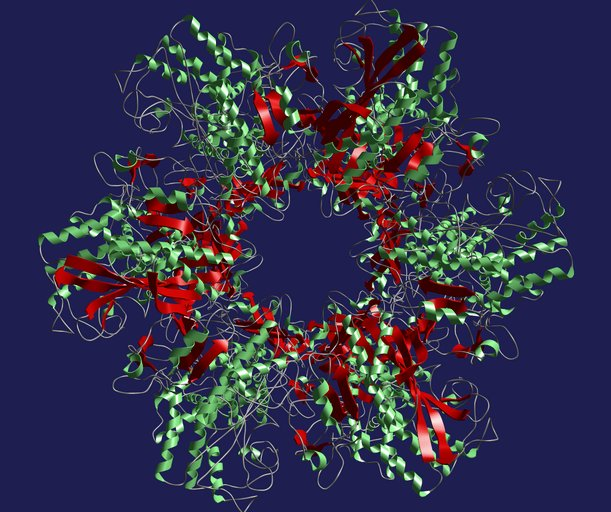
\includegraphics[scale=0.33]{scp/008.jpg}
\end{center}

\fakebold{Special Containment Procedures:} SCP-008 samples are extreme biological hazards and all related protocols apply. Incineration and irradiation measures will be deployed in the event of political or military action which may result in the facility being dismantled; a power failure; or zero communications from operatives or outside channels during any given eight (8)-hour period. The quarantine period for operatives leaving the facility is four (4) months. If a breach has occurred, incineration and irradiation measures shall be deployed. It should be the policy of all G2 sites to not prepare an evacuation procedure.

\fakebold{Description:} SCP-008 is a complex prion, samples of which are stored in each of the known G2 sites. Research into SCP-008 is highly classified and primarily aimed at preventing research which may lead to the synthesis of SCP-008 in the distant future. Traits of the SCP-008 prion include:
\begin{itemize}
\renewcommand{\labelitemi}{$\ast$}
\item 100\% infectiousness.
\item 100\% lethality.\newpage
\item Transmission through exposed mucous membranes and all bodily fluids.
\item Not airborne or waterborne.
\end{itemize}
Symptoms of infection with SCP-008 manifest no more than three hours after exposure, and include:
\begin{itemize}
\renewcommand{\labelitemi}{$\ast$}
\item Flu-like symptoms with high fever, plus severe dementia in later stages.
\item Coma onset approximately 20 hours after first symptoms appear and 12 hours after noticeable dementia. Coma onset will be considered onset of death.
\item A period of sporadic cellular necrosis occurs which comes to resemble gangrene. \item Surviving tissue assumes its original function and is highly resilient.
\item Red blood cells greatly increase oxygen storage capacity, resulting in slower blood flow and increased muscle endurance and strength.
\item Nervous and muscular systems are unaffected by total organ failure for several hours.
\item Metabolism may decrease to extremely low levels, allowing subject to survive for over 10 years without nutrition.
\item High blood viscosity results in negligible blood flow from gunshot, puncture, and slashing injuries.
\item Conditioned behavior, motor controls, and instinctive behavioral mechanisms are damaged, and cognitive abilities are severely retarded and erratic. Animals experience excessive brain necrosis and are inactive.
\item Subject can adapt to its damaged nervous systems but is limited to basic physical activities, including standing up, balancing on two legs, walking, biting, grabbing, and crawling. Subject will energetically move towards sights, sounds, and smells it associates with living humans. Subject will attempt to ingest living humans if physical contact is made.
\item Neutralizing fully-infected subjects requires significant cranial trauma.
\end{itemize}
There is strong evidence to suggest SCP-008 itself did not form naturally on Earth, since variants of similar complexity would have displaced much of the ecosystem. In 1959, a short collaborative effort with the USSR to locate G2 sites and eliminate SCP-008 was negotiated following their discovery. The status of SCP-008 in Russian custody since collaboration ended is unknown.

\fakebold{Addendum 008-1:} SCP-500 has been found to be able to completely cure SCP-008 even in the advanced stages of the disease.